\chapter*{Input/Output}
\addcontentsline{toc}{chapter}{Input/Output}


\section*{Concepts}
\addcontentsline{toc}{section}{Concepts}

Twin-64 features memory a mapped I/O architecture.


memory mapped

dedicated address space in physical memory

bus concept 

module concept

modules have registers - load / store, however registers do not have to be 64 bit wide.

the system bus features up to 64 modules. that is: 64 HPA pages, need: 1Mb address range.

a module listens to three address ranges

- hard physical address range. a page. privileged.

- soft physical address range. allocated by the module for further space. aligned on a page boundary.

- broadcast address range. Mirrors the system bus range. A write to a register in that range applies to all corresponding registers of a module on the same bus. 

modules are processors, memory and I/O cards.

we could keep processor stats in the HPA space

memory module has entire memory as SPA space


\section*{I/O Address Space}
\addcontentsline{toc}{section}{I/O Address Space}

 As shown in the overall physical memory layout, the physical memory address range dedicated to I/O modules is located from \texttt{0x00\_F000\_0000} to \texttt{0x00\_FFFF\_FFFF}. The following figure depicts the I/O memory address space ranges in more detail.s

\begin{figure}[H]
\begin{center}
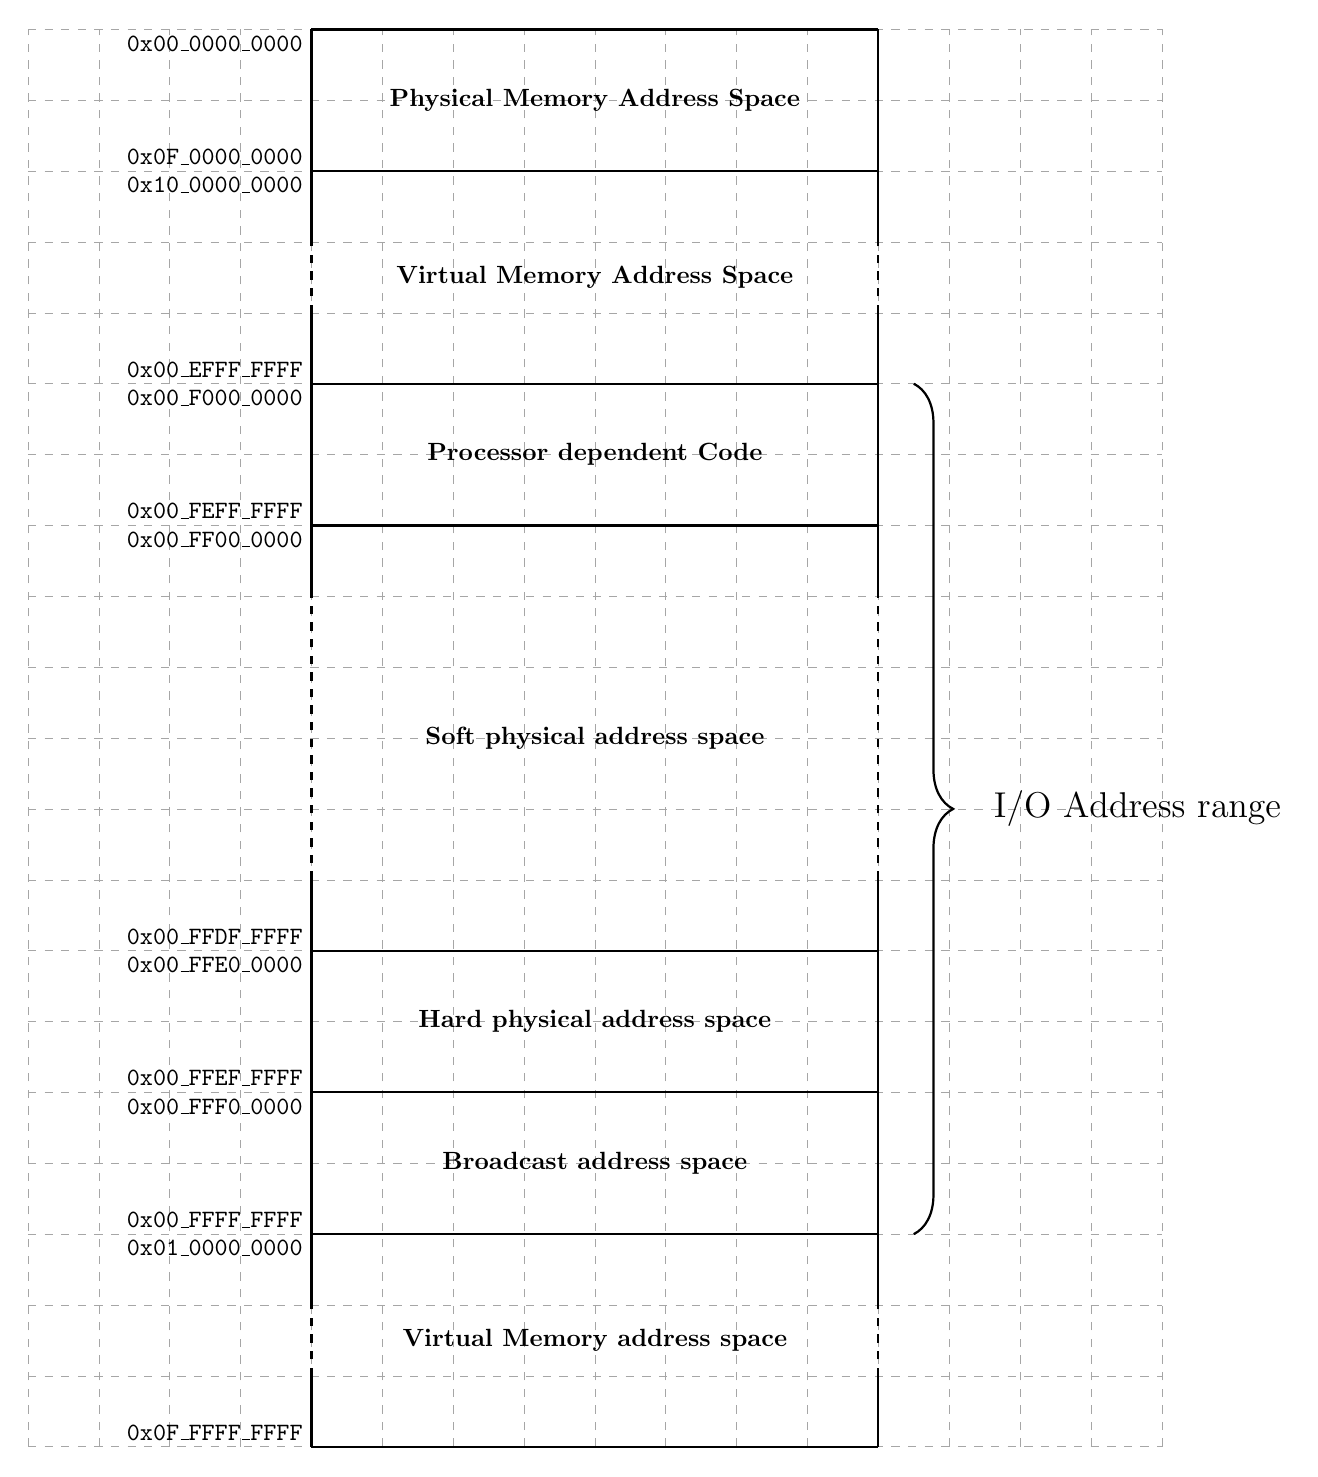
\begin{tikzpicture}[scale=0.9, transform shape]
        
  	\draw[help lines, gray!70, dashed] (0,0) grid(16,20);

	% Rectangle dimensions
	\def\width{8}
	\def\leftofs{4}
	\def\rightofs{\leftofs + \width}

	% Left side
	\draw[thick] (\leftofs, 0) -- (\leftofs, 1); 
	\draw[thick, dashed] (\leftofs, 1) -- (\leftofs, 2);
	\draw[thick] (\leftofs, 2) -- (\leftofs, 8); 
	\draw[thick, dashed] (\leftofs, 8) -- (\leftofs, 12);
	\draw[thick] (\leftofs, 12) -- (\leftofs, 16);
	\draw[thick, dashed] (\leftofs, 16) -- (\leftofs, 17);
	\draw[thick] (\leftofs, 17) -- (\leftofs, 18);
	\draw[thick] (\leftofs, 18) -- (\leftofs, 20);

	% Right side
	\draw[thick] (\rightofs, 0) -- (\rightofs, 1); 
	\draw[thick, dashed] (\rightofs, 1) -- (\rightofs, 2);
	\draw[thick] (\rightofs, 2) -- (\rightofs, 8); 
	\draw[thick, dashed] (\rightofs, 8) -- (\rightofs, 12);
	\draw[thick] (\rightofs, 12) -- (\rightofs, 16); 	
	\draw[thick, dashed] (\rightofs, 16) -- (\rightofs, 17);
	\draw[thick] (\rightofs, 17) -- (\rightofs, 18); 
	\draw[thick] (\rightofs, 18) -- (\rightofs, 20); 
		
	% Edges
	\draw[thick] (\leftofs, 0) -- (\rightofs, 0); 
	\draw[thick] (\leftofs, 3) -- (\rightofs, 3); 
	\draw[thick] (\leftofs, 5) -- (\rightofs, 5); 
	\draw[thick] (\leftofs, 7) -- (\rightofs, 7);
	\draw[thick] (\leftofs, 13) -- (\rightofs, 13);
	\draw[thick] (\leftofs, 15) -- (\rightofs, 15);
	\draw[thick] (\leftofs, 18) -- (\rightofs, 18);
	\draw[thick] (\leftofs, 20) -- (\rightofs, 20);

	% Labels 
	\node[left] at (\leftofs, 20 - 0.2) {\texttt{0x00\_0000\_0000}};
	\node[left] at (\leftofs, 18 + 0.2) {\texttt{0x0F\_0000\_0000}};
	\node[left] at (\leftofs, 18 - 0.2) {\texttt{0x10\_0000\_0000}};
	\node[left] at (\leftofs, 15 + 0.2) {\texttt{0x00\_EFFF\_FFFF}};
	\node[left] at (\leftofs, 15 - 0.2) {\texttt{0x00\_F000\_0000}};
	\node[left] at (\leftofs, 13 + 0.2) {\texttt{0x00\_FEFF\_FFFF}};
	\node[left] at (\leftofs, 13 - 0.2) {\texttt{0x00\_FF00\_0000}};
	\node[left] at (\leftofs, 7 + 0.2) {\texttt{0x00\_FFDF\_FFFF}};
	\node[left] at (\leftofs, 7 - 0.2) {\texttt{0x00\_FFE0\_0000}};
	\node[left] at (\leftofs, 5 + 0.2) {\texttt{0x00\_FFEF\_FFFF}};
	\node[left] at (\leftofs, 5 - 0.2) {\texttt{0x00\_FFF0\_0000}};
	\node[left] at (\leftofs, 3 + 0.2) {\texttt{0x00\_FFFF\_FFFF}};
	\node[left] at (\leftofs, 3 - 0.2) {\texttt{0x01\_0000\_0000}};
	\node[left] at (\leftofs, 0 + 0.2) {\texttt{0x0F\_FFFF\_FFFF}};
		
	\node at (\leftofs + \width / 2, 19) {\textbf{Physical Memory Address Space}};
	\node at (\leftofs + \width / 2, 16.5) {\textbf{Virtual Memory Address Space}};
	\node at (\leftofs + \width / 2, 14) {\textbf{Processor dependent Code}};
	\node at (\leftofs + \width / 2, 10) {\textbf{Soft physical address space}};
	\node at (\leftofs + \width / 2, 6) {\textbf{Hard physical address space}};
	\node at (\leftofs + \width / 2, 4) {\textbf{Broadcast address space}};
	\node at (\leftofs + \width / 2, 1.5) {\textbf{Virtual Memory address space}};
	
	% bracket
	\draw[thick]  [decorate, decoration={brace, amplitude=0.5cm, mirror}] (\rightofs + 0.5,3) -- (\rightofs + 0.5,15)
	node[midway, right=1cm, anchor=west]{\Large I/O Address range};
	

\end{tikzpicture}
\end{center}
\caption{I/O Memory Address Range}
\label{fig:I/O Memory Address Range}
\end{figure}

The I/O address range is a 256Mbyte area in the first 4 Gbyte segment, i.e.segment 0. The area is divided into several ranges. The first range contains the processor dependent code. There is a set of library functions to manage the processor itself but also provide low-level primitives for the boot process and the operating system. 

\section*{Hard physical address range}
\addcontentsline{toc}{section}{Hard physical address range}

The \textbf{hard physical address} range contains a I/O page for each I/O modules installed. There room for 64 I/O modules.

\section*{Broadcast address range}
\addcontentsline{toc}{section}{Broadcast address range}

The \textbf{broadcast address} range mirrors the hard physical address range. However, a write to these locations is a write operation to which all I/O modules will react.

\section*{Soft physical address range}
\addcontentsline{toc}{section}{Soft physical address range}

The \textbf{soft physical address} range is an area where space is allocated to an I/O module. The I/O module reacts to a memory access operation in its configured soft physical address range.

\section*{I/O Elements}
\addcontentsline{toc}{section}{I/O Elements}

I/O elements are 128 bytes, i.e. 16 regs 

I/O elements can also be two pages, one priv and one user level, mapped...




